% 第5章第2节：核与函数空间的构造（从半正定核构造空间、特征映射、核的运算）。

\section{核与函数空间的构造}
\label{sec:rkhs-construction}

上一节从空间出发得到了核，并看到每个再生核都是半正定核。本节回答反方向的问题：只给定集合$X$上的一个半正定核，能否找到以它为再生核的函数空间，这个空间是否唯一。第~\ref{sec:rkhs-from-kernel}节用核截面的有限组合、商去零长度方向和完备化三步给出一般构造。一般构造虽然完整，却不便于检验一个具体的二元函数是否半正定，所以后两小节给出两种可操作的办法：把核写成特征向量的内积，或者由已知的核经运算得到新核。这些步骤都只用到集合与核，不需要预先给定测度。

\subsection{从半正定核构造空间}
\label{sec:rkhs-from-kernel}

设$K$是非空集合$X$上的半正定核。如果以$K$为再生核的空间存在，它一定含有全部核截面$K_x$，并且核截面之间的内积必须是$\langle K_x,K_z\rangle=K(z,x)$。构造就从这两点出发。

\paragraph{有限核和与它们的内积}

令$H_0=\operatorname{span}\{K_x:x\in X\}$，它由有限和$f=\sum_{i=1}^na_iK_{x_i}$组成，每个元素都是$X$上的真实函数$f(t)=\sum_ia_iK(t,x_i)$。对$f=\sum_ia_iK_{x_i}$与$g=\sum_jb_jK_{z_j}$，按照上述要求定义
\begin{equation}
\langle f,g\rangle_0=\sum_{i,j}a_ib_jK(z_j,x_i).
\label{eq:rkhs-h0-inner}
\end{equation}

同一个函数可以有多种有限和表示，必须先检查式~\eqref{eq:rkhs-h0-inner}与表示的选取无关。对$j$先求和内层的$i$，得到$\langle f,g\rangle_0=\sum_jb_jf(z_j)$，它只依赖于$f$作为函数的取值；由$K$的对称性，同一个量也等于$\sum_ia_ig(x_i)$，只依赖于$g$的取值。于是换掉$f$的表示不改变第一种写法，换掉$g$的表示不改变第二种写法，$\langle f,g\rangle_0$良定义。它显然对称、双线性，且$\langle f,f\rangle_0=\bm a^{\top}\bm G\bm a\ge0$，其中$\bm G$是点组$x_1,\ldots,x_n$上的Gram矩阵。取$g=K_x$，由第一种写法立刻得到
\begin{equation}
\langle f,K_x\rangle_0=f(x)\qquad(f\in H_0),
\label{eq:rkhs-h0-reproducing}
\end{equation}
即再生性质在$H_0$上已经成立。

\paragraph{零长度方向}

若把系数向量$\bm a$本身当作对象，二次型$\bm a^{\top}\bm G\bm a$只是半正定的，可能对非零$\bm a$取零。第~\ref{sec:rkhs-kernel-properties}节的仿射核例子中，点$-1,0,1$上的系数$(1,-2,1)$长度为零。所以不能直接把系数空间连同这个二次型当作内积空间，必须先商去零长度的方向。

把系数映成函数，恰好完成了这个商。Cauchy--Schwarz不等式的证明只用到半正定性与双线性，对$\langle\cdot,\cdot\rangle_0$同样成立，结合式~\eqref{eq:rkhs-h0-reproducing}得
\begin{equation}
|f(x)|=|\langle f,K_x\rangle_0|\le\sqrt{K(x,x)}\,\|f\|_0 .
\label{eq:rkhs-h0-point-bound}
\end{equation}
所以长度为零的组合在每一点取零，是零函数；反过来，零函数$f$满足$\langle f,f\rangle_0=\sum_ia_if(x_i)=0$。零长度的系数组合恰好就是给出零函数的组合。在仿射核的例子中，$K_{-1}-2K_0+K_1$正是零函数。因此在函数空间$H_0$上，$\langle\cdot,\cdot\rangle_0$已经是真正的内积。

\paragraph{完备化与点值的极限}

$H_0$一般不完备。为得到Hilbert空间，取$H_0$的完备化$\overline{H_0}$：由定理~\ref{thm:metric-completion}，它由$H_0$中Cauchy列的等价类组成，内积可以由连续性延拓过去（第~\ref{sec:fs-hilbert}节）。但完备化中的元素是抽象的等价类，还不是$X$上的函数，接下来要把它们变回函数。

点值估计~\eqref{eq:rkhs-h0-point-bound}正好提供了这一步。若$(f_n)$是$H_0$中的Cauchy列，则$|f_n(x)-f_m(x)|\le\sqrt{K(x,x)}\|f_n-f_m\|_0$，所以在每一点$f_n(x)$都是Cauchy数列，有确定的极限；等价的Cauchy列相差一列趋于零的函数，在每一点有相同的极限。用内积表达，就是定义
\[
J:\overline{H_0}\to\{X\text{上的实函数}\},\qquad (J\xi)(x)=\langle\xi,K_x\rangle_{\overline{H_0}} .
\]
若$f_n\to\xi$，则$f_n(x)=\langle f_n,K_x\rangle\to(J\xi)(x)$，所以$J\xi$就是逼近$\xi$的Cauchy列的逐点极限；由式~\eqref{eq:rkhs-h0-reproducing}，$J$在$H_0$上是恒等映射。

\paragraph{排除额外的零方向}

还剩一个危险：$\overline{H_0}$中两个不同的元素，会不会给出同一个函数？若是这样，函数之间就无法定义内积。等价地，要排除这样的$\xi\neq0$：$J\xi$是零函数。这一步要用到核截面在$\overline{H_0}$中稠密。若$(J\xi)(x)=\langle\xi,K_x\rangle=0$对一切$x$成立，则$\xi$与每个$K_x$正交，从而与它们的张成$H_0$正交；$H_0$在$\overline{H_0}$中稠密，所以$\xi$与整个空间正交，$\xi=0$。因此$J$是单射。

\begin{theorem}[由半正定核确定再生核Hilbert空间]
\label{thm:rkhs-moore-aronszajn}
设$K$是非空集合$X$上的半正定核。则存在唯一的RKHS，记为$H_K$，以$K$为其再生核。并且有限核和全体$H_0=\operatorname{span}\{K_x:x\in X\}$在$H_K$中稠密，$H_K$的每个元素都是$H_0$中某个Cauchy列的逐点极限。
\end{theorem}

\begin{proof}
存在性。令$H_K=J(\overline{H_0})$，并规定$\langle J\xi,J\eta\rangle_{H_K}=\langle\xi,\eta\rangle_{\overline{H_0}}$。由于$J$是线性单射，这个定义良好，且$J$成为从$\overline{H_0}$到$H_K$的等距同构，所以$H_K$是Hilbert空间；$J$的线性说明$H_K$中的加法和数乘就是逐点运算。$J$在$H_0$上是恒等映射，故$K_x=JK_x\in H_K$，并且对$f=J\xi$有
\[
f(x)=\langle\xi,K_x\rangle_{\overline{H_0}}=\langle J\xi,JK_x\rangle_{H_K}=\langle f,K_x\rangle_{H_K} .
\]
这就是以$K$为再生核的再生性质，点值有界随之成立。稠密性与逐点极限的描述来自$H_0$在$\overline{H_0}$中稠密以及上一段关于$J$的讨论。

唯一性。设$H$是另一个以$K$为再生核的RKHS。$H$含有每个$K_x$，且$\langle K_x,K_z\rangle_H=K(z,x)$，所以$H_0\subseteq H$，两者在$H_0$上的内积一致。$H_0$在$H$中也稠密：若$f\in H$与每个$K_x$正交，则由再生性质$f(x)=0$对一切$x$成立。任取$f\in H$及$H_0$中的序列$f_n\to f$（按$H$的范数），$(f_n)$是$H_0$中的Cauchy列，再生性质说明它逐点收敛到$f$；同一序列在$H_K$中收敛到其逐点极限，即$f$。所以$f\in H_K$且$\|f\|_{H_K}=\lim\|f_n\|=\|f\|_H$。对调两个空间的角色，得$H=H_K$，且范数相同。
\end{proof}

这条结论通常称为Moore--Aronszajn定理\scite{aronszajn1950kernels}。图~\ref{fig:rkhs-construction-steps}概括了四个阶段：系数组合上只有半内积；变为函数后零长度方向被商去；完备化补上极限；点值读取把极限元素重新表示为函数，核截面的稠密性保证这种表示是单射。

\begin{figure}[!htb]
  \centering
  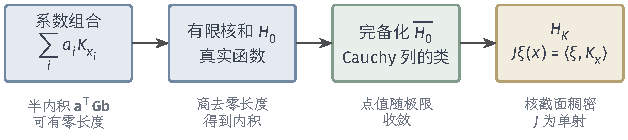
\includegraphics[width=106.4mm]{figures/02-abstract-mathematics/03-function-spaces/tikz/c5-construction-steps/figure.pdf}
  \caption{由半正定核构造$H_K$的四个阶段。系数组合上的二次型$\bm a^{\top}\bm G\bm b$只是半内积，可能有零长度方向；把组合看成函数便商去了这些方向，得到内积空间$H_0$；完备化$\overline{H_0}$的元素是Cauchy列的类，点值估计使它们的点值随极限收敛；映射$J$把它们表示为函数，核截面稠密保证$J$为单射。}
  \label{fig:rkhs-construction-steps}
\end{figure}

\paragraph{由最小值核重建$H_{\min}$}

以最小值核为例走一遍构造。$H_0$由$\min(\cdot,x_j)$的有限组合组成，即在$[0,1]$上连续、分段线性、左端为零、在最右节点之后保持常数的函数。核截面的内积可以写成导数的积分：
\[
\langle K_x,K_z\rangle_0=\min(x,z)=\int_0^1\mathbf 1_{[0,x]}(t)\mathbf 1_{[0,z]}(t)\,\mathrm dt=\int_0^1K_x'(t)K_z'(t)\,\mathrm dt ,
\]
所以在$H_0$上$\|f\|_0=\|f'\|_{L^2}$。$H_0$中函数的导数恰好是阶梯函数，而区间上的阶梯函数在$L^2(0,1)$中稠密（第~\ref{sec:fs-density-separability}节），于是完备化后得到的空间经由$f\mapsto f'$与$L^2(0,1)$等距同构，它就是第~\ref{sec:rkhs-reproducing}节的$H_{\min}$。$H_0$本身不完备：例如$f(t)=t-t^2/2$属于$H_{\min}$，却不是分段线性函数，它只是$H_0$中一列折线的极限。

这个例子也说明了唯一性的用处：我们已经知道$H_{\min}$是以$\min(x,z)$为再生核的RKHS，定理~\ref{thm:rkhs-moore-aronszajn}立刻保证从核出发构造的空间就是它，不必另作比较。

\paragraph{构造用到了什么}

整个构造只用到集合$X$与核的半正定性，没有测度，也不要求$X$带有拓扑。所得的稠密性是在核范数意义下：$H_K$中的每个函数都能被有限核和按$\|\cdot\|_{H_K}$逼近，因而也被逐点逼近。这并没有回答有限核和能否逼近$H_K$之外的函数，例如$[0,1]$上任意给定的连续函数；那是第~\ref{sec:apx-kernel-sections}节要讨论的问题，答案取决于具体的核。

\subsection{特征映射}
\label{sec:rkhs-feature-maps}

一般构造告诉我们半正定核总对应一个空间，但要验证某个二元函数半正定，逐一检查所有Gram矩阵并不现实。最常用的办法是把核写成两个向量的内积。

\paragraph{有限特征向量的内积核}

设$\Phi:X\to\mathbb R^d$，令$K(x,z)=\Phi(x)^{\top}\Phi(z)$。对任意点组与系数，
\[
\sum_{i,j}a_ia_jK(x_i,x_j)=\Bigl\|\sum_ia_i\Phi(x_i)\Bigr\|_2^2\ge0 ,
\]
所以$K$是半正定核；用矩阵写，Gram矩阵等于$\bm\Phi\bm\Phi^{\top}$，其中$\bm\Phi$的第$i$行是$\Phi(x_i)^{\top}$。例如，对实数$x,z$，
\[
(1+xz)^2=1+2xz+x^2z^2=\bigl\langle(1,\sqrt2\,x,x^2),\ (1,\sqrt2\,z,z^2)\bigr\rangle ,
\]
所以二次多项式核是三维特征向量的内积核。

\paragraph{一般特征映射}

有限维的要求可以去掉。

\begin{definition}[特征映射]
\label{def:rkhs-feature-map}
设$X$是非空集合，$\mathcal F$是实Hilbert空间，$\Phi:X\to\mathcal F$是任意映射。若$K(x,z)=\langle\Phi(x),\Phi(z)\rangle_{\mathcal F}$，则称$\Phi$为$K$的一个\term{特征映射}（feature map），$\mathcal F$为相应的特征空间。
\end{definition}

与有限维情形完全相同的计算说明，任何特征映射给出的$K$都是半正定核。反过来，每个半正定核都有特征映射：取$\mathcal F=H_K$、$\Phi(x)=K_x$，则$\langle K_x,K_z\rangle_{H_K}=K(x,z)$。称它为\term{规范特征映射}（canonical feature map）。所以“$K$半正定”与“$K$有某个特征映射”是等价的。

同一个核可以有许多不同的特征映射。仿射核$1+xz$既可以写成$\Phi_1(x)=(1,x)\in\mathbb R^2$的内积，也可以写成$\Phi_2(x)=(1,x/\sqrt2,x/\sqrt2)\in\mathbb R^3$的内积，因为$1+\tfrac{x z}{2}+\tfrac{xz}{2}=1+xz$。特征空间的维数和坐标都可以不同，核却相同，因此由核确定的空间也相同。下面说明这个空间怎样从任何一个特征映射读出来。

\paragraph{参数表示与可见子空间}

给定特征映射$\Phi:X\to\mathcal F$，每个参数$w\in\mathcal F$确定一个函数
\[
f_w(x)=\langle w,\Phi(x)\rangle_{\mathcal F}.
\]
令$V=\overline{\operatorname{span}}\{\Phi(x):x\in X\}$为特征值张成的闭子空间，$P_V$为到$V$的正交投影。由于$w-P_Vw$与每个$\Phi(x)$正交，$f_w=f_{P_Vw}$：正交补$V^\perp$中的参数分量不影响函数。称$V$为可见参数子空间。

\begin{theorem}[特征映射给出的RKHS]
\label{thm:rkhs-feature-space}
设$\Phi:X\to\mathcal F$是半正定核$K$的特征映射，$V$为特征值张成的闭子空间。则
\[
H_K=\{f_w:w\in\mathcal F\},\qquad
\|f_w\|_{H_K}=\|P_Vw\|_{\mathcal F}=\min_{u\in\mathcal F,\ f_u=f_w}\|u\|_{\mathcal F} ,
\]
并且$w\mapsto f_w$限制在$V$上是从$V$到$H_K$的等距同构。
\end{theorem}

\begin{proof}
线性映射$A:w\mapsto f_w$的核是$\{w:\langle w,\Phi(x)\rangle=0,\ \forall x\}=V^\perp$，所以$A$在$V$上是单射。令$H=A(\mathcal F)=A(V)$，并规定$\|Aw\|_H=\|P_Vw\|$，则$A|_V$是等距同构，$H$作为闭子空间$V$的等距像是Hilbert空间，运算是逐点的。

点值有界：$|f_w(x)|=|\langle P_Vw,\Phi(x)\rangle|\le\|\Phi(x)\|\,\|f_w\|_H$。再生核：令$k_x=A\Phi(x)$，因$\Phi(x)\in V$，有$\langle f_w,k_x\rangle_H=\langle P_Vw,\Phi(x)\rangle=f_w(x)$；而$k_x(z)=\langle\Phi(x),\Phi(z)\rangle=K(z,x)$，即$k_x=K_x$。所以$H$是以$K$为再生核的RKHS，由定理~\ref{thm:rkhs-moore-aronszajn}的唯一性，$H=H_K$。最后，$f_u=f_w$当且仅当$u-w\in V^\perp$，此时$P_Vu=P_Vw$，而$\|u\|\ge\|P_Vu\|$，等号在$u\in V$时取得。
\end{proof}

定理的最后一个等式提醒我们：在冗余的特征表示中，任意一个能给出$f$的参数$w$，其范数只是$\|f\|_{H_K}$的上界；只有落在可见子空间中的那一个参数，范数才等于函数的范数。

\paragraph{冗余特征的例子}

取$\Phi(x)=(x,x)\in\mathbb R^2$，核为$K(x,z)=2xz$。可见子空间是直线$V=\operatorname{span}\{(1,1)\}$，正交补方向是$(1,-1)$。参数$(2,0)$、$(1,1)$、$(0,2)$都给出同一函数$f(x)=2x$，范数分别为$2$、$\sqrt2$、$2$；由定理~\ref{thm:rkhs-feature-space}，$\|f\|_{H_K}=\sqrt2$，它是$(2,0)$在$V$上的投影$(1,1)$的长度，见图~\ref{fig:rkhs-visible-parameters}。直接检验：$H_K$由$f(x)=cx$组成，核截面$K_x(t)=2xt$，再生性质要求$\langle ct,2xt\rangle=cx$，故$\langle ct,c't\rangle_{H_K}=cc'/2$，$\|2x\|_{H_K}^2=4/2=2$，结果一致。

对仿射核的两个特征映射，$\Phi_1$的可见子空间是整个$\mathbb R^2$（$\Phi_1(-1)$与$\Phi_1(1)$线性无关），所以$\|a+bt\|_{H_K}^2=a^2+b^2$，与第~\ref{sec:rkhs-reproducing}节一致。$\Phi_2$的可见子空间是$\operatorname{span}\{(1,0,0),(0,1,1)/\sqrt2\}$，参数$(a,b/\sqrt2,b/\sqrt2)$给出$a+bt$，长度同样是$\sqrt{a^2+b^2}$；而参数$(a,\sqrt2 b,0)$给出同一函数，长度$\sqrt{a^2+2b^2}$却更大。

\begin{figure}[!htb]
  \centering
  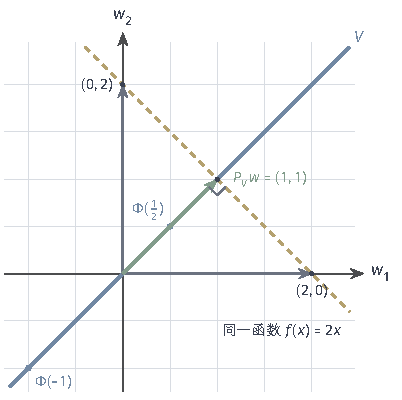
\includegraphics[width=68.1mm]{figures/02-abstract-mathematics/03-function-spaces/tikz/c5-visible-parameters/figure.pdf}
  \caption{冗余特征$\Phi(x)=(x,x)$的参数平面。特征值$\Phi(x)$都落在蓝色直线$V$上；黄色虚线上的参数都给出同一函数$f(x)=2x$。其中与$V$相交的$P_Vw=(1,1)$长度最短，为$\sqrt2$，这就是$\|f\|_{H_K}$；$(2,0)$与$(0,2)$长度为$2$，多出的部分来自对函数没有影响的$V^\perp$方向。}
  \label{fig:rkhs-visible-parameters}
\end{figure}

\subsection{核的运算}
\label{sec:rkhs-kernel-operations}

特征映射适合验证可以写成内积的核。更多的核是由几种基本核经过加法、乘法和换输入等运算得到的；只要这些运算保持半正定性，就不必为每个新核重新寻找特征映射。

\paragraph{保持半正定性的运算}

\begin{theorem}[核的运算]
\label{thm:rkhs-kernel-operations}
设$K_1,K_2$是非空集合$X$上的半正定核。则下列函数都是半正定核：
\begin{enumerate}
\item 非负线性组合$\alpha K_1+\beta K_2$，其中$\alpha,\beta\ge0$；
\item 逐点乘积$K_1(x,z)K_2(x,z)$；
\item 换输入：对任意集合$Y$和映射$\varphi:Y\to X$，$Y$上的$K_1(\varphi(y),\varphi(y'))$；
\item 函数缩放：对任意$g:X\to\mathbb R$，$g(x)g(z)K_1(x,z)$；
\item 逐点极限：若半正定核$K^{(n)}$在每个$(x,z)$处收敛到$K(x,z)$，则$K$半正定。
\end{enumerate}
\end{theorem}

\begin{proof}
固定点组$x_1,\ldots,x_n$与系数向量$\bm c$，记$\bm G_1,\bm G_2$为两个核的Gram矩阵。第1条：$\bm c^{\top}(\alpha\bm G_1+\beta\bm G_2)\bm c=\alpha\bm c^{\top}\bm G_1\bm c+\beta\bm c^{\top}\bm G_2\bm c\ge0$；用特征映射表达，把$\sqrt\alpha\,\Phi_1(x)$与$\sqrt\beta\,\Phi_2(x)$拼接成直和空间中的一个向量即可。

第2条：乘积核的Gram矩阵是逐元素乘积$\bm G_1\odot\bm G_2$。半正定矩阵$\bm G_2$可分解为$\bm G_2=\bm B\bm B^{\top}$（例如由谱分解取$\bm B=\bm U\bm\Lambda^{1/2}$），记$\bm b_k$为$\bm B$的第$k$列，则
\[
\bm c^{\top}(\bm G_1\odot\bm G_2)\bm c
=\sum_{i,j}c_ic_j(\bm G_1)_{i,j}\sum_k\bm B_{i,k}\bm B_{j,k}
=\sum_k(\bm c\odot\bm b_k)^{\top}\bm G_1(\bm c\odot\bm b_k)\ge0 .
\]
这就是Schur乘积定理。若两个核分别有有限维特征映射，乘积核的特征映射是张量积$\Phi_1(x)\otimes\Phi_2(x)$，因为$\langle u\otimes v,u'\otimes v'\rangle=\langle u,u'\rangle\langle v,v'\rangle$。

第3条：点组$y_1,\ldots,y_n$上的Gram矩阵就是点组$\varphi(y_1),\ldots,\varphi(y_n)$上$K_1$的Gram矩阵（允许点重复）。第4条：二次型等于$(\bm c\odot\bm g)^{\top}\bm G_1(\bm c\odot\bm g)$，其中$\bm g=(g(x_1),\ldots,g(x_n))$。第5条：每个二次型$\bm c^{\top}\bm G^{(n)}\bm c$非负，有限和的极限仍非负。
\end{proof}

逐元素乘积的半正定性和张量积的内积公式都是有限维线性代数中的结论，可参考\BookChapterRef{chap:normed-inner-product-spaces}{卷一《数学准备：基础数学》“赋范空间与内积空间”章中的Gram矩阵与Schur乘积}及\BookChapterRef{chap:linear-operations}{卷一“向量、矩阵与张量的运算”章中的张量积}。这里只用到它们在有限点组上的形式。

\paragraph{线性核、多项式核与高斯核}

由这几条规则可以验证常用的核。在$\mathbb R^d$上，\term{线性核}$K(\bm x,\bm z)=\bm x^{\top}\bm z$以$\Phi(\bm x)=\bm x$为特征映射。常数$c\ge0$是以$\sqrt c$为特征的核，于是$c+\bm x^{\top}\bm z$半正定（第1条），它的$p$次幂即\term{多项式核}$(c+\bm x^{\top}\bm z)^p$也半正定（第2条反复使用）。

\term{高斯核}（Gaussian kernel）$K_\sigma(\bm x,\bm z)=\exp\bigl(-\|\bm x-\bm z\|_2^2/(2\sigma^2)\bigr)$分三步验证。先把指数中的平方展开：
\[
\exp\Bigl(-\frac{\|\bm x-\bm z\|_2^2}{2\sigma^2}\Bigr)
=g(\bm x)\,g(\bm z)\,\exp\Bigl(\frac{\bm x^{\top}\bm z}{\sigma^2}\Bigr),\qquad
g(\bm x)=\exp\Bigl(-\frac{\|\bm x\|_2^2}{2\sigma^2}\Bigr).
\]
再看中间的因子：对每个$N$，部分和$\sum_{k=0}^N(\bm x^{\top}\bm z)^k/(k!\,\sigma^{2k})$是线性核的幂的非负组合，因而半正定；指数级数在每一点收敛，由第5条，极限$\exp(\bm x^{\top}\bm z/\sigma^2)$半正定。最后由第4条乘上$g(\bm x)g(\bm z)$。

\paragraph{运算在核截面上的效果}

核运算直接作用在核截面上：和核的截面是两个截面之和，乘积核的截面是两个截面之积。图~\ref{fig:rkhs-kernel-operations}在$x=0.4$处比较仿射核与高斯核（$\sigma=0.3$）。和核的截面在仿射趋势上叠加了一个局部隆起；乘积核的截面仍集中在$x$附近，但被仿射因子$1+0.4t$拉得右高左低。这说明乘积核所对应空间中的函数同时带有两种核的特点：局部性来自高斯因子，倾斜来自仿射因子。

\begin{figure}[!htb]
  \centering
  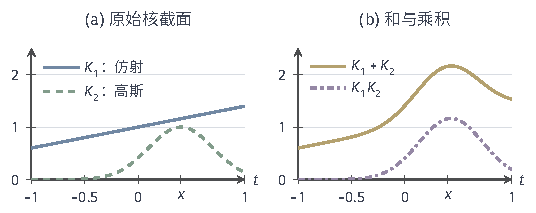
\includegraphics[width=90.7mm]{figures/02-abstract-mathematics/03-function-spaces/tikz/c5-kernel-operations/figure.pdf}
  \caption{核运算在核截面上的效果，固定$x=0.4$，$t\in[-1,1]$。(a)~仿射核截面$1+0.4t$与高斯核截面（$\sigma=0.3$）；(b)~两者之和与逐点乘积。和核的截面是两个截面相加，乘积核的截面是两个截面相乘，仍保持以$x$为中心的局部形状。}
  \label{fig:rkhs-kernel-operations}
\end{figure}

\paragraph{半正定性给不出的结论}

上面的规则只涉及非负组合、乘积与极限，减法不在其中。两个半正定核之差一般不是半正定核：仿射核减去常数核$2$得到$xz-1$，它在$x=z=0$处的对角值为$-1$，而半正定核的对角值$K(x,x)$必须非负。

半正定性也不包含更强的性质。二次多项式核$(1+xz)^2$在$\mathbb R$上半正定，但由特征映射$(1,\sqrt2x,x^2)$与定理~\ref{thm:rkhs-feature-space}，它的RKHS就是至多二次的多项式全体，任意四个点上的Gram矩阵都奇异，所以它不是严格正定核。这个三维空间在$C[-1,1]$中是闭的，不能一致逼近$|x|$这样的连续函数。高斯核既严格正定，又能用有限核和逼近紧区间上的任意连续函数，但后一性质需要第~\ref{sec:apx-kernel-sections}节专门的稠密性论证，不能从半正定性推出。
